% !TEX root = ../dissertacao.tex
\chapter{Trabalhos correlatos}
\label{cap:trabalhos_correlatos}

Este capítulo revisa os principais trabalhos de otimização do uso da memória cache.
Inicialmente, na Seção~\ref{sec:trabalhos_cache_aware} serão abordados os trabalhos correlatos que consideram informações da arquitetura da memória cache (\textit{cache-aware}).
Posteriormente, na Seção~\ref{sec:trabalhos_cache_oblivous} serão abordados os trabalhos que desprezam informações sobre a arquitetura de memória cache em que o programa será executado (\textit{cache-oblivious}).
Por fim, na Seção~\ref{sec:analise_trabalhos_correlatos}, será apresentado um resumo do estado da arte e suas oportunidades de contribuições científicas.
É importante ressaltar que este capítulo não faz uma análise exaustiva de cada trabalho citado, mas busca apresentar as características mais relevantes das principais abordagens para otimização do uso da memória cache.

\section{Trabalhos correlatos considerando \textit{cache-aware}}
\label{sec:trabalhos_cache_aware}

Esta seção apresenta os trabalhos correlatos que consideram o modelo de \textit{cache-aware}.
Algoritmos \textit{cache-aware} são aqueles que possuem informações sobre a arquitetura da cache a priori.
Com estas informações estes trabalhos buscam otimizar seus comportamentos para extrair o máximo de desempenho de uma dada arquitetura.
Como por exemplo, uma multiplicação de matrizes pode ser realizada em blocos para melhorar a localidade da cache.

\begin{figure}[hb]
    \centering
    \subfigure[$1^a$ iteração]{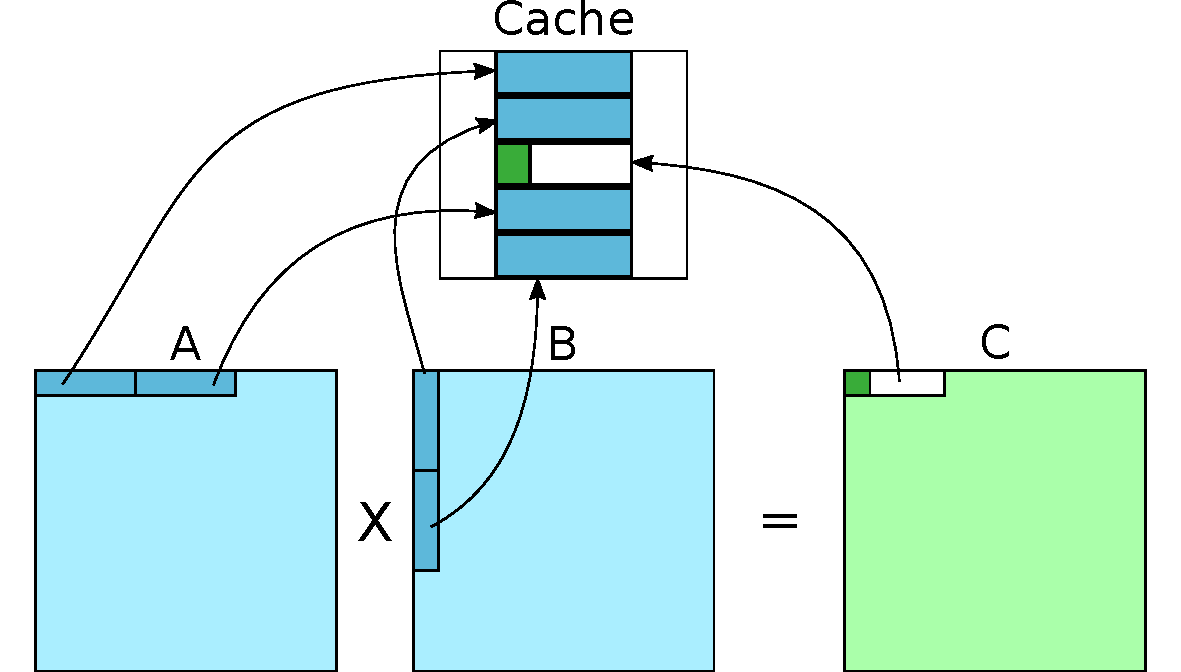
\includegraphics[width=0.3\linewidth]{img/multiplicacao_matrix_a}}
    \subfigure[$2^a$ iteração]{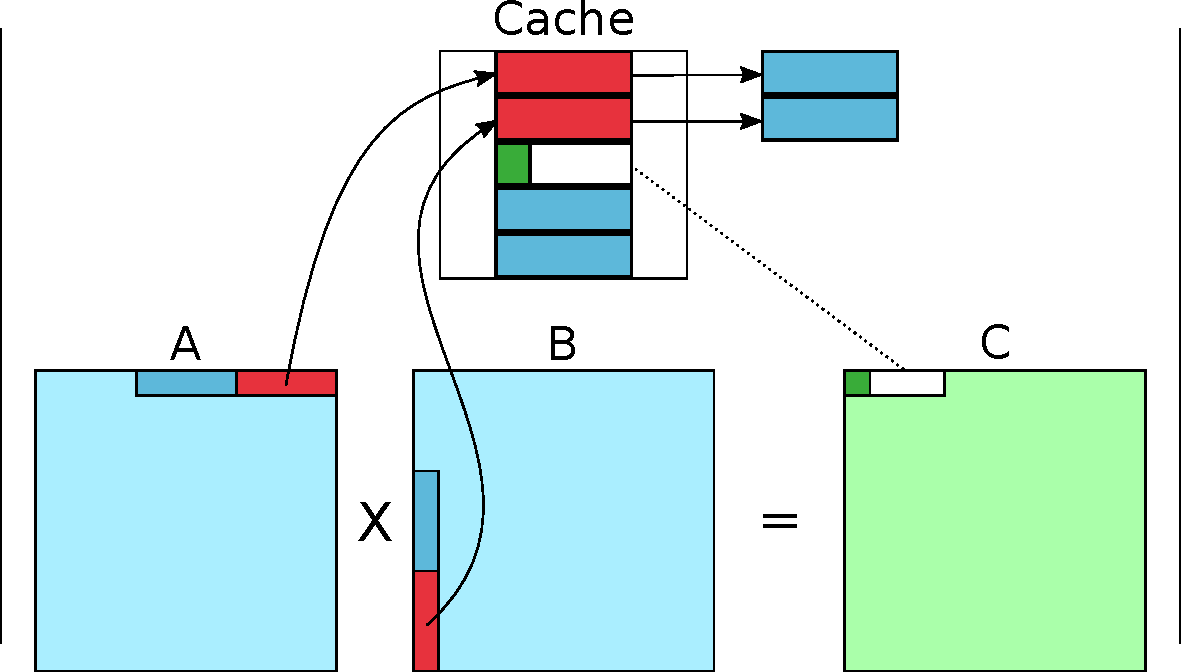
\includegraphics[width=0.3\linewidth]{img/multiplicacao_matrix_b}}
    \subfigure[$3^a$ iteração]{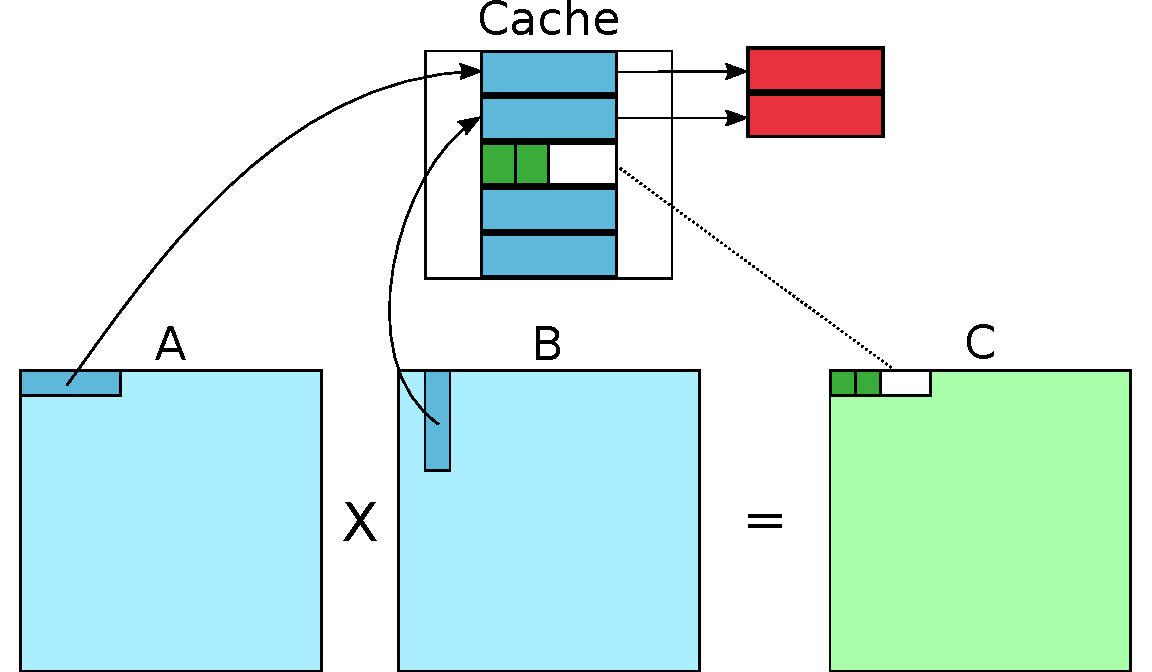
\includegraphics[width=0.3\linewidth]{img/multiplicacao_matrix_c}}
    \caption[Exemplo multiplicação de matrizes]{Exemplo multiplicação de matrizes com abordagem tradicional.}
    \label{fig:multiplicacao_matriz}
\end{figure}

A Figura~\ref{fig:multiplicacao_matriz} apresenta como seria uma multiplicação de duas matrizes utilizando a abordagem tradicional. Nesta figura, os \textit{cache misses} são representados pelas setas e a linha pontilhada representa um \textit{cache hit}. Podemos notar que os blocos carregados para a cache não são reaproveitados no passo seguinte da multiplicação, o que irá gerar um grande aumento no numero de instruções executadas bem como no tempo toral de execução.

Um algoritmo \textit{cache aware} para a multiplicação de matrizes poderia tirar proveito do conhecimento do tamanho do bloco da cache para executar as operações em uma sub-matriz.
A multiplicação de matrizes em blocos é possível uma vez que esta operação é apenas uma enorme adição de uma pilha de produtos, não importando qual ordem estas adições são realizadas.
O único cuidado que se deve tomar neste caso é para que todos os produtos sejam realizados corretamente e contribuam para as somas adequadas.

\begin{figure}[hb]
    \centering
    \subfigure[$1^a$ iteração]{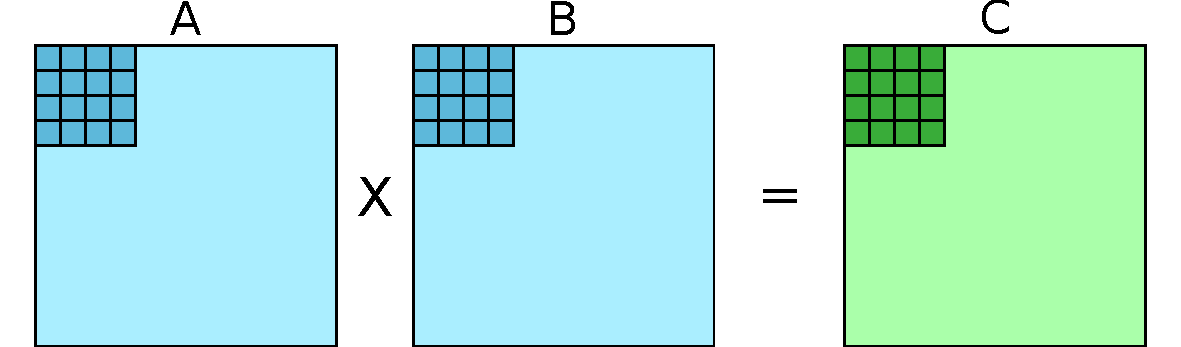
\includegraphics[width=0.3\linewidth]{img/multiplicacao_matrix_bloco_a}}
    \subfigure[$2^a$ iteração]{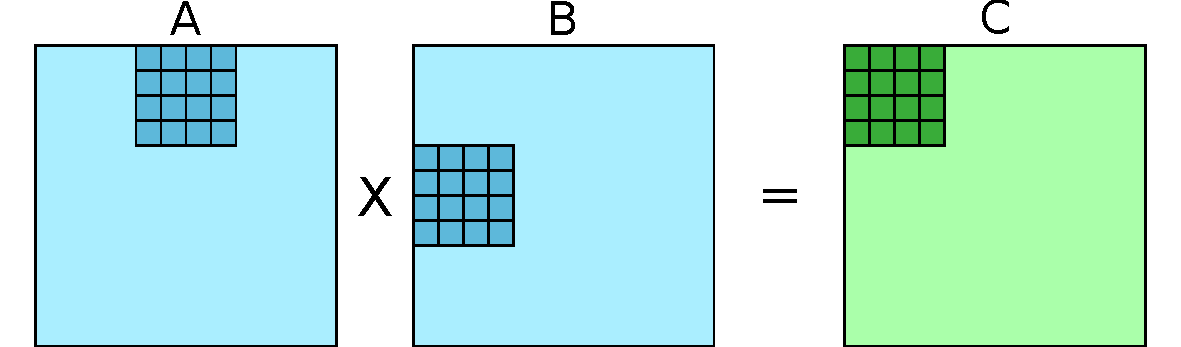
\includegraphics[width=0.3\linewidth]{img/multiplicacao_matrix_bloco_b}}
    \subfigure[$3^a$ iteração]{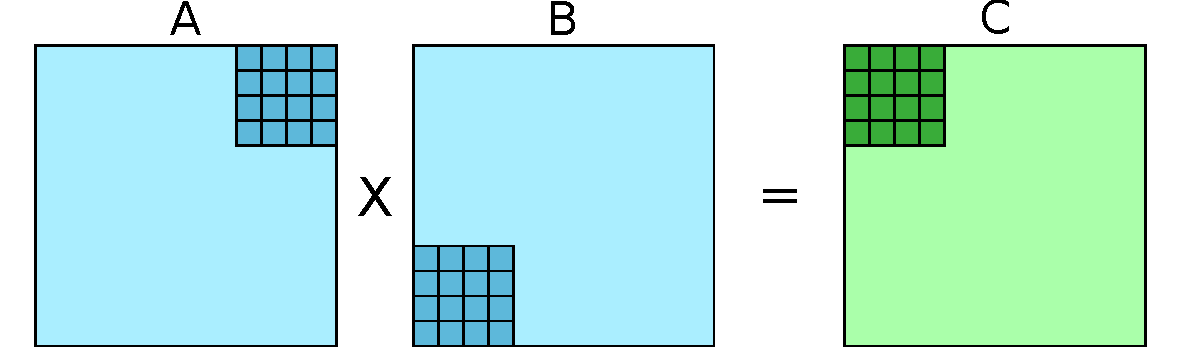
\includegraphics[width=0.3\linewidth]{img/multiplicacao_matrix_bloco_c}}
    \caption[Exemplo multiplicação de matrizes em blocos]{Exemplo multiplicação de matrizes em blocos.}
    \label{fig:multiplicacao_matriz_bloco}
\end{figure}

A Figura~\ref{fig:multiplicacao_matriz_bloco} ilustra a execução de um algoritmo \textit{cache aware} de multiplicação de matrizes. Por ter conhecimento do tamanho do bloco da cache em que este algoritmo será executado, são executadas operações de submatrizes de tamanho $4 \times 4$. Esta otimização faz com que o número de \textit{cache misses} seja reduzido drasticamente, uma vez que o bloco recuperado para a cache é totalmente utilizado.

% Um desses trabalhos tem como enfoque a modelagem da arquitetura perante um conjunto de aplicações.

% \subsection{\citeonline{DiazAlvarez2016}}

% O trabalho de \citeonline{DiazAlvarez2016} visa encontrar a melhor configuração de uma arquitetura cache para um conjunto pré definido de aplicações.
% O contexto deste trabalho inclui aplicações para dispositivos móveis e portanto, operados a bateria.
% Seu principal objetivo é reduzir o tempo de execução das aplicações, bem como, o consumo energético demandado pelas mesmas.
% Para determinar as arquiteturas, este trabalho visa encontrar a capacidade, tamanho do bloco e associatividade da cache.

% \citeonline{DiazAlvarez2016} tomaram como base o trabalho de \citeonline{wang2012dynamic}.
% \citeonline{wang2012dynamic} realizaram uma análise combinando análise estática e dinâmica para determinar as configurações da cache para sistemas embarcados de tempo real.
% Com isso, \citeonline{wang2012dynamic} minimizam o consumo de energia em até $74\%$.

% Para determinar as arquiteturas, \citeonline{DiazAlvarez2016} encontraram os parâmetros da cache baseados em \ac{ge}~\cite{dempsey2009foundations} utilizando \textit{tracers} e determinando a configuração baseado-se no tempo de execução e consumo de energia.
% Esta técnica garante uma redução no tempo de execução pois o algoritmo meta-heurístico converge mesmo com um curto número de gerações e tamanho da população; e a técnica adiciona um \textit{hash} para armazenar os valores objetivos de cada cache avaliada.
% Para avaliar o trabalho, foram utilizados os \textit{benchmarks} Mediabench~\cite{mediabench1997}.
% Esta técnica conseguiu reduzir o tempo de execução em $75\%$ em média, e obteve $96\%$ de redução de consumo de energia em média.

\subsection{\citeonline{majeti2013compiler}}

O trabalho de \citeonline{majeti2013compiler} possui como objetivo principal determinar o melhor leiaute dos dados para um determinado programa. Segundo o autor, o leiaute ideal para um programa computacional depende de se o mesmo é executado em um núcleo de CPU, uma GPU discreta, ou em uma GPU integrada (juntamente com outros fatores). Com isso, para obter programas que extraíssem todo o potencial de uma arquitetura, seria necessário rescrever o código fonte para cada arquitetura de CPU\@/\@GPU.

Para sanar o problema da reescrita do código para cada arquitetura, \citeonline{majeti2013compiler} propõem a inserção de metadados nos códigos-fonte. Estes metadados guiariam um compilador a selecionar as melhores estruturas de dados para uma dada arquitetura de CPU\@/\@GPU. Com isso, o compilador é capaz de escolher e converter os dados de \ac{aos} para \ac{soa} e vice-versa.
% Neste trabalho também é apresentado que a escolha do leiaute dos dados que maximiza o número de acessos coalescidos (acessos que utilizam o mesmo bloco da cache e, portanto, minimizam o número de cache misses) em uma GPU é NP-completo~\cite{wu2013complexity}.
Majeti et al. ainda ressaltam que os metadados se fazem necessários pois a escolha de um leiaute de dados que maximiza o número de acessos coalescidos (acessos que utilizam o mesmo bloco da cache e, portanto, minimizam o número de cache misses) para uma GPU é NP-completo. A prova que esta escolha é da classe NP-completo foi realizada por~\citeonline{wu2013complexity}.


Para avaliar a eficiência da técnica de compilação proposta, os autores geraram \textit{benchmarks} sintéticos e avaliaram a execução compilando esses códigos com e sem os metadados. Em algumas arquiteturas como AMD 4-core A10-5880K CPU e NVIDIA Tesla M2050 GPU conseguiram um \textit{speedup}\footnote{A métrica \textit{speedup} representa a relação entre os tempos de execução da solução sequencial e a solução paralela para um determinado número de threads.} de até $27,11 \times$ e $29,50 \times$ respectivamente.

\section{Trabalhos correlatos considerando \textit{cache-oblivious}}
\label{sec:trabalhos_cache_oblivous}

Esta seção apresenta os trabalhos correlatos que consideram o modelo de \textit{cache-oblivious}.
Algoritmos \textit{cache-oblivious} (ou \textit{cache-tran\-scen\-dent}) são algoritmos projetados para explorar a memória cache de uma CPU sem ter o tamanho da mesma (ou o tamanho das linhas, etc.) como um parâmetro explícito~\cite{frigo1999cache}. Assim, um algoritmo \textit{cache-oblivious} é concebido para funcionar otimizadamente, sem modificação, em inúmeras arquiteturas com diferentes tamanhos de cache, ou para uma hierarquia de memória com diferentes níveis de cache e tamanhos variados.

\subsection{\citeonline{li2014}}

O trabalho de \citeonline{li2014} tem como enfoque o gerenciamento da cache compartilhada em processadores multi-core.
Segundo o autor, a gestão do compartilhamento de cache não é apenas para alcançar um bom desempenho, mas também para garantir um desempenho estável em um ambiente dinâmico; e considerando não apenas programas paralelos, mas também programas sequenciais co-executados uns com os outros.

Para identificar onde o gerenciamento da cache pode incidir, os autores descrevem um método para reorganizar o código para um leiaute ideal com base no \ac{pdg}.
Com estas informações, é construído um \ac{trg}~\cite{gloy1999procedure} para otimizar o leiaute do código em tempo de compilação.
A otimização realiza duas transformações: reordenamento global das funções e\@/\@ou reordenamento dos blocos inter-procedurais. Estes reordenamentos são baseados na afinidade do acesso à cache.

Para mensurar suas otimizações, os autores utilizaram os \textit{benchmarks} SPEC CPU 2006~\cite{spec2006}, realizando os experimentos tanto em uma máquina real como em um simulador de instruções da cache. Para medir a proporção de cache misses, utilizaram contadores de desempenho de hardware.
O método melhorou o desempenho de todos os programas em até $3\%$ quando estes foram executados separadamente (somente um programa por processador).
Quando executados mais de um programa por processador, este método obteve até $10,3\%$ de melhoria. Ao utilizar melhor a cache compartilhada, o método amplia a melhoria da transferência de \textit{hiper-threading} em $8\%$.

\subsection{\citeonline{Tang2015}}

O trabalho de \citeonline{Tang2015} visa preservar a localidade da cache em algoritmos de Programação Dinâmica no contexto de algoritmos cache-oblivious paralelos.
% Estes algoritmos geralmente aplicam estratégias de divisão e conquista recursivamente, o que assintoticamente atinge o uso ótimo da localidade temporal de uma cache sequencial.
Estes algoritmos geralmente subdividem o problema em instâncias menores, o que assintoticamente atinge o uso ótimo da localidade temporal de uma cache sequencial.
No entanto, o escalonamento das tarefas pela granularidade de suas dependências limita o paralelismo ao introduzir dependências artificiais entre subtarefas recursivas, além das decorrentes das equações de recorrência~\cite{Tang2015}.

Para realizar as otimizações, \citeonline{Tang2015} removeram as dependências artificiais. Com isso, foi possível agendar as tarefas prontas para execução assim que todas as restrições reais de dependência eram satisfeitas (instruções atômicas foram usadas para identificar e iniciar tarefas prontas). Assim, eles conseguiram preservar a otimização da cache herdada da estratégia de dividir e conquistar.
Com a paralelização e remoção das dependências artificiais, Tang et al. atingiram uma melhoria de 3 a 5 vezes no tempo absoluto de execução.

\subsection{\citeonline{qasem2017characterizing}}

% O trabalho de \citeonline{qasem2017characterizing} caracteriza o impacto no desempenho da organização dos dados em arquiteturas de \ac{hpc} com sistemas de memória heterogêneos e de vários níveis.

Segundo os autores, este é o primeiro trabalho a considerar a organização dos dados juntamente com o leiaute da memória.
\citeonline{qasem2017characterizing} caracterizam os problemas de desempenho com a organização de dados em arquiteturas de memória heterogêneas, visando descobrir os cenários aos quais seria rentável realizar uma reorganização das estruturas de dados compartilhadas para uma maior desempenho.
Segundo o autor, a eficiência do acesso aos dados é impactada pelos padrões de acesso à memória, leiaute da estrutura de dados e características do caminho sobre o qual os dados serão transferidos entre o processador e a unidade de memória.

Com base no estudo realizado sobre os efeitos das organização de dados tradicionais para sistemas de memória heterogêneos, como \ac{aos} e \ac{soa}, os autores propõem uma nova estrutura de dados denominada \ac{ca}.
Esta estrutura de dados se comporta tanto como \ac{aos} ou \ac{soa}, dependendo do tipo de acesso a dados que está sendo realizado.
As decisões sobre a organização dos dados considera três atributos principais: \textit{register pressure}, intensidade aritmética e esparsidade no acesso aos dados.

O estudo realizado por \citeonline{qasem2017characterizing} demonstrou que a abordagem de utilizar \ac{soa} nem sempre é lucrativa e que a escolha da organização dos dados deve considerar uma variedade de fatores, incluindo intensidade aritmética e esparsidade no acesso aos dados.
A nova estratégia de organização dos dados (\ac{ca}), que aborda as limitações das abordagens atuais (\ac{aos} e \ac{soa}), atingiu uma aceleração de uma ordem de magnitude em algumas arquiteturas.

\section{Análise qualitativa dos trabalhos correlatos}
\label{sec:analise_trabalhos_correlatos}

Esta seção apresenta uma análise dos trabalhos correlatos citados neste capítulo.
A Tabela~\ref{tab:resumo_trabalhos_correlatos} classifica os trabalhos correlatos de acordo com o modelo de memória cache utilizado (\textit{Cache-Aware} ou \textit{Cache-Oblivious}) e o momento em que a otimização ocorre.
Ela também identifica os casos de usos que foram utilizados em cada um dos trabalhos.


% Please add the following required packages to your document preamble:
% \usepackage{booktabs}
% \usepackage{lscape}
\begin{table}[hb]
\centering
\caption{Resumo dos trabalhos correlatos.}
\label{tab:resumo_trabalhos_correlatos}
\resizebox{\textwidth}{!}{%
\begin{tabular}{@{}cccc@{}}
\toprule
Trabalho      & Consideração da Cache & Momento da Otimização & Casos de Uso                                                               \\ \midrule
% Álvarez, 2016 & Cache-Aware           & N/A                   & Mediabench                                                                 \\
Majeti, 2013  & Cache-Aware           & Compilação            & sintéticos                                                                 \\
Li, 2014      & Cache-Oblivious       & Compilação            & SPEC2006 CPU                                                               \\
Tang, 2015    & Cache-Oblivious       & Pós-Compilação        & sintéticos                                                                 \\
Qasem, 2017   & Cache-Oblivious       & Pós-Compilação        & sintéticos                                                                 \\
Este Trabalho & Cache-Oblivious       & Pré-Compilação        & \begin{tabular}[c]{@{}c@{}}3 algoritmos de\\ Physical Design*\end{tabular} \\ \midrule
\multicolumn{4}{l}{* Entrada realista oriunda de circuitos industriais providos pela competição ICCAD2015 \cite{kim2015}.}                
\end{tabular}
}
\end{table}

Diversos métodos de otimizações já foram avaliados, dentre os quais se destacam:
heurísticas para selecionar estrutura de dados realizado por \citeonline{majeti2013compiler};
\citeonline{li2014} reorganizou as instruções baseando-se em grafo de dependências;
\citeonline{sung2010data} realizou conversão das estruturas de dados para aumentar a utilização da cache compartilhada empregando transformações em tempo de compilação.
Porém, a grande maioria destes trabalhos avaliam seus resultados com \textit{benchmarks} sintéticos e nenhum destes trabalhos considera o contexto de \textit{Physical Design}.

Não foram localizados trabalhos que considerassem otimizações de software para \textit{cache-oblivious} no contexto de \textit{Physical Design}.
Portanto este trabalho possui como principal diferencial a aplicação de técnicas de otimizações no contexto de \textit{Physical Design}.
Estas otimizações serão implementadas numa biblioteca \textit{open source} para ensino e pesquisa de síntese física chamada Ophidian~\cite{ophidian}.
Este trabalho aborda o modelo de \textit{Cache-Oblivious} por ser uma biblioteca \textit{open source}                                                                                                                                                                e as otimizações carecem suportar diversas arquiteturas.
Para avaliar os 3 algoritmos de \textit{Physical Design} considerando um senário realista, este trabalho irá utilizar circuitos industriais providos para a análise do problema C da competição ICCAD 2015 CAD Contest~\cite{kim2015}.
